\documentclass{amsart}

\usepackage{amsmath, amsthm, amssymb} %AMS math

\usepackage{graphicx}% Include figure files
\usepackage{bm}% bold math
\usepackage{color} % colored text
\usepackage[pdftex,colorlinks=true,
allcolors=blue
]{hyperref}% add hypertext capabilities
\usepackage{paralist}% for compactitem used by Marko
\usepackage{multirow}% multicolumn/row cells in tables

\usepackage{url} % add auto-linked urls
\usepackage{mathtools} % shortintertext, and other useful math-related features
\usepackage{siunitx}
\sisetup{per-mode = symbol}
\usepackage[dvipsnames]{xcolor}
\usepackage{listings} % including code
\usepackage{amsrefs} % references

\graphicspath{{figs/}} % store figures in figs subfolder

% packages for plotting directly in MATLAB
\usepackage{pgfplots}
\pgfplotsset{compat=newest}
\usepackage{braids} % plotting braids


%% comments
\newcommand{\marko}[1]{\textcolor{red}{(MB: {\bfseries #1})}}
\newcommand{\reese}[1]{\textcolor{red}{(ARM: {\bfseries #1})}}

\begin{document}

\title{Title of our paper}

\author{A. Reese Madsen III}
\address{Department of Mathematics, Clarkson University,
Potsdam, NY}
\email{madsenar@clarkson.edu}

\author{Marko Budi\v{s}i\'c}
\address{Department of Mathematics, Clarkson University,
Potsdam, NY}
\email{mbudisic@clarkson.edu}
\urladdr{http://people.clarkson.edu/~mbudisic} % Delete if not wanted.

\begin{abstract}
Great stuff.
\end{abstract}

\maketitle % typeset the title page
\tableofcontents % table of contents

\section{Introduction}

\begin{itemize}
\item motivation for the problem
\item discussion of existing results in literature, covering all aspects of the paper
\item announcement of the original contribution
\item short outline of the paper sections (Section 1 does this, Section 2 does that, etc.)
\end{itemize}

\section{Problem description}

\begin{figure}[htb]
  \centering
  \begin{center}
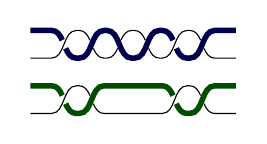
\begin{tikzpicture}
  \braid[rotate=-90,
  width=10pt, % spacing between strands
  height=10pt, % size of element of the braid (crossing)
  style strands={1}{blue!30!black,line width=2pt},
  style strands={2}{blue!30!black,black},
  style strands={3}{green!30!black,line width=2pt},
  style strands={4}{green!30!black,black}]
  s_1-s_3 s_1-s_3 s_1 s_1^{-1}  s_1-s_3 s_1-s_3;
\end{tikzpicture}
\end{center}
\caption{This is how you plot braids in a paper.}\label{fig:braids}
\end{figure}


\begin{itemize}
\item describe what a braid is
\item describe what a brownian motion is and what a brownian bridge is
\item describe how a brownian bridge can be used to create a braid (conceptually)
\item formulate the research question: ``We are trying to understand \dots in dependence of parameters \dots.''
\end{itemize}

\section{Main technique}

\begin{itemize}
\item how do we create (simulate) strands -- describe exactly what MATLAB's \texttt{bm} does
\item how do we convert strands into a braid -- refer to papers and documentation of \texttt{braidlab} to see how this is done
\item how are calculations you're performing on any braid defined (entropy, length, etc.) --- this does not have to be very in-depth, but it should be accurate
\item what parameters we have chosen to vary between braids; what parameters stay fixed? why?
\item how are you creating your ensembles of braids (especially if we're using the subsampling of a large braid)
\end{itemize}

\section{Results with Commentary}

Graphs with commentary. This section should be neatly organized so that the readers don't have a too difficult time following what parameters change, what are fixed, etc.

For behaviors that can be explained succinctly, do so. E.g. ``entropy increases with the length of braid'' can be explained succinctly. On the other hand ``entropy follows the formula \(f(N)\)'' needs more justification. Point out that the deeper discussion of such questions will be in the discussion section and/or that we do not have a good way of accounting for such behavior.

\section{Discussion and Conclusions}



\bibliography{bibliography} % bibliography.bib stores references

\appendix

\section{How to use LaTeX?}

Example of notes. Some math $\int_0^Tx(t)dt$. If you'd like to put an equation in its own line, this is how you do it:
\begin{equation}
x(t) = x_0 + \int_0^T f(x(\tau))d\tau  \label{eq:ode-solution}
\end{equation}


You can also refer to an equation that you made, if you gave it a label, just like this \eqref{eq:ode-solution}.

If you want to include an image, this is how you do it. And you can also refer to the Figure~\ref{fig:graph}.
\begin{figure}
  \centering
  \includegraphics[width=0.2\linewidth]{figs/graph.png}
  \caption{This is a graph.}\label{fig:graph}
\end{figure}

\textbf{  All the help you need is found here: \url{https://en.wikibooks.org/wiki/LaTeX}. }


You can create a bulleted list
\begin{itemize}
\item First
\item Second
\item Third
\end{itemize}


\begin{figure}
  \includegraphics[width=0.5\linewidth]{figs/graph.png}
  \caption{Image}
\end{figure}
You can also enumerate
\begin{enumerate}
\item First
\item Second
\item Third
\end{enumerate}

If you want a tighter itemization, use \verb|compactitem| and \verb|compactenum|
\begin{compactitem}
\item First
\item Second
\item Third
\end{compactitem}

\begin{compactenum}
\item First
\item Second
\item Third
\end{compactenum}

Most people get matrices wrong (overly complicated) in \LaTeX. This is the right way:
\[ %this produces unenumerated equation.
  \begin{bmatrix}
    1 & 2 \\
    \ast & 3
  \end{bmatrix}
\]
More details are here:
\url{https://en.wikibooks.org/wiki/LaTeX/Mathematics\#Matrices_and_arrays}.


LaTeX (with help of pgfplot) can also create graphs of functions.
\begin{figure}[htb]\centering
   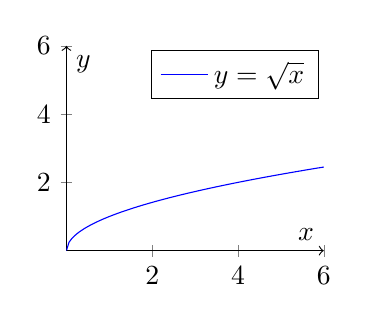
\begin{tikzpicture}
     \begin{axis}[
       xmin=0, xmax=6,
       xlabel={$x$},
       ymin=0, ymax=6,
       ylabel={$y$},
       axis lines=middle,
       axis line style=->,
       width=.4\textwidth
     ]
       \addplot[no marks,blue,-,domain=0:6, samples=100] expression{sqrt(x)};
       \addlegendentry{$y=\sqrt{x}$};
     \end{axis}
   \end{tikzpicture}
 \end{figure}

 This is how you include some code\footnote{For more see \url{https://www.overleaf.com/learn/latex/Code_listing\#Using_listings_to_highlight_code}.}:
\begin{lstlisting}[language=Matlab]
for k = 2:9
    u[k] = u[k-1] - 2*u[k] + u[k+1];
end
\end{lstlisting}

Figure~\ref{fig:csvfig} was made purely in \LaTeX.\footnote{For more such plots see \url{http://pgfplots.sourceforge.net/gallery.html}}

\begin{figure}[htb]
  \centering
  \begin{tikzpicture}
\begin{axis}[width=0.8\linewidth, height=0.55\linewidth,
  enlargelimits=0.15,
  xmin=-5,xmax=5, mark size=1.5pt,
  legend pos = north west, legend style={fill=none,draw=none},
  yticklabel style={/pgf/number format/.cd,fixed,precision=2},
  xlabel={Value}, ylabel={Proportion} % labels
  ]
  \addplot+ table[x=Value, y=Proportion, col sep=comma]{figs/dataset.csv};
\end{axis}
\end{tikzpicture}
\caption{Graph made directly in LaTeX.}\label{fig:csvfig}
\end{figure}

Example of a cited paper \cite{Hill1894}.

 Some \textbf{important formatting tips}:
\begin{compactitem}
\item Please make sure to use operator notation (with backslashes) when appropriate.\footnote{\url{https://en.wikibooks.org/wiki/LaTeX/Mathematics\#Operators}}
\item There's a lot of bad advice on how to write matrices. Here's the correct way: \url{https://en.wikibooks.org/wiki/LaTeX/Mathematics\#Matrices_and_arrays}
\item Mixing text and equations is another sore spot: \url{https://en.wikibooks.org/wiki/LaTeX/Mathematics\#Adding_text_to_equations}
\item Tidy multiline equations (use \verb|align| instead of \verb|eqnarray|)\footnote{This is an official guidance from TeX community \url{https://texfaq.org/FAQ-eqnarray}} \url{https://en.wikibooks.org/wiki/LaTeX/Advanced_Mathematics\#align_and_align.2A}
\item Annotating parts of equations using braces \url{https://en.wikibooks.org/wiki/LaTeX/Advanced_Mathematics\#Above_and_below}
\item Never use manual linebreak \verb|\\| in text (outside \verb|align|,\verb|bmatrix| and other similar multiline formula environments). If you think you need it, you're wrong.\footnote{\url{https://en.wikibooks.org/wiki/LaTeX/Paragraph_Formatting\#Manual_breaks}} Instead use an empty line (to break a paragraph), or displayed equations using a pair of \verb|$$| or \verb|\[|,\verb|\]| (preferred).
\end{compactitem}


\end{document}
